\section{Design}\label{sec: Design}
In this section the design and decisions that where made to achieve the laboratory are discussed.
%The code for lab 03 can be reviewed online under the flowing link \href{https://github.com/haringd/EGR680_FPGA_Labs/tree/master/VENDMACH}{http://github.com/haringd/EGR680\_FPGA\_Labs/tree/master/VENDMACH}.
\subsection{SDK Lab specification}\label{subsec: Vending machine specification}
In this part, you will create a simple hardcore ARM Cortex-A9 based embedded system on the PYNQ board. The
embedded system design is broken up into three parts: Hardware design of the ARM Cortex-A9 hardcore
processor, application software design using SDK, and finally hardware implementation of the software running
on the hardcore processor. The application you will design in this part is a UART application that prints “HELLO
WORLD” to a terminal emulator like Tera Term. Use the figure below as a flow guide for this lab. The diagram
for the completed design is shown in Figure \ref{fig: Vivado_lab4_CompletedDesign}. 
\begin{figure}[H]
	\centering
	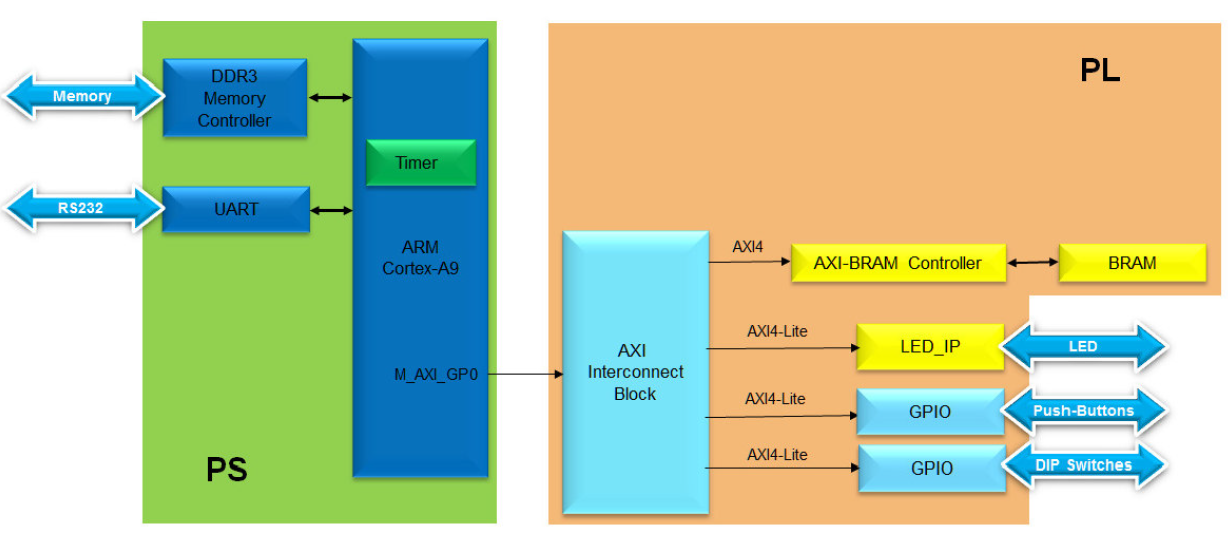
\includegraphics[width=1.0\textwidth]{01_images/Vivado_lab4_CompletedDesign.PNG}
	\caption{Completed Design.}
	\label{fig: Vivado_lab4_CompletedDesign}
\end{figure}

\subsection{HDL}\label{subsec: HDL}
Figure \ref{fig: Vivado_lab_HDL_topView} shows the HDL top level based of the ZYNQ 7 Processing system which is connected with an AXI bus S00\_AXI to a intellectual property (IP) block that manages peripherals. From there an AXI bus is used to connect two general purpose input output (GPIO) IP blocks, one for buttons and another one for switches. Furthermore, a Processor System Reset IP block is used that interconnects all resets.
\begin{figure}[H]
	\centering
	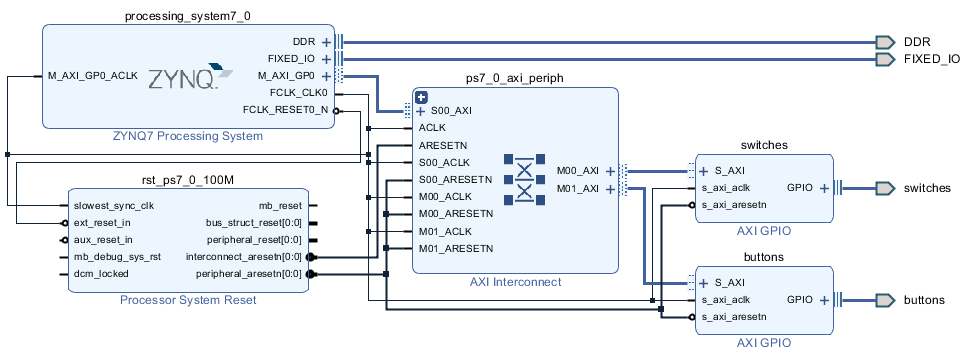
\includegraphics[width=1.0\textwidth]{01_images/Vivado_lab_HDL_topView.PNG}
	\caption{HDL Top Level Design.}
	\label{fig: Vivado_lab_HDL_topView}
\end{figure}

\subsection{SDK}\label{subsec: SDK}
After the HDL top level is defined the SDK can be launched with \textbf{File $\rightarrow$ Launch SDK}. The *.hdf file should be shown or can be opened that shows the base registers for the switches and buttons, as highlighted in Figure \ref{fig: Vivado_lab4_SW_BTN_Register}. 
\begin{figure}[H]
	\centering
	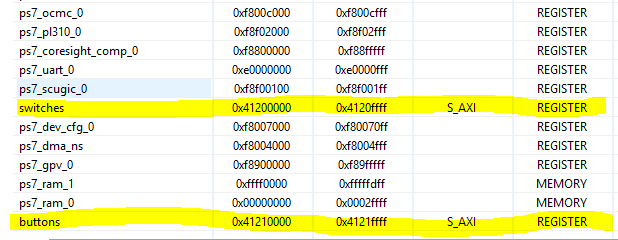
\includegraphics[width=1.0\textwidth]{01_images/Vivado_lab4_SW_BTN_Register.PNG}
	\caption{*.hdf file that shows the base register for switches and buttons.}
	\label{fig: Vivado_lab4_SW_BTN_Register}
\end{figure}

After writing the C code given in part two and loading the the bit stream file and the build elf file onto the board the serial console Terra Term shows the status of the buttons and switches, as shown in Figure \ref{fig: Vivado_lab4_TT_PartII}
\begin{figure}[H]
	\centering
	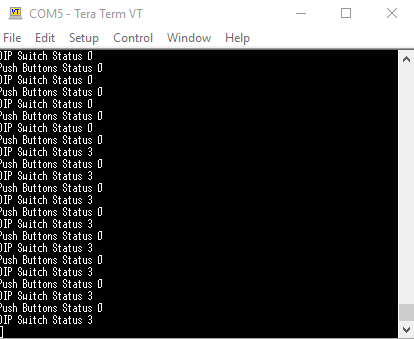
\includegraphics[width=0.7\textwidth]{01_images/Vivado_lab4_TT_PartII.PNG}
	\caption{Terra Term print out of the switches and buttons status.}
	\label{fig: Vivado_lab4_TT_PartII}
\end{figure}

\subsection{Let's Make a Deal}\label{subsec: Lets Make a Deal}


\subsection{Errors}\label{subsec: Errors}
\begin{figure}[H]
	\centering
	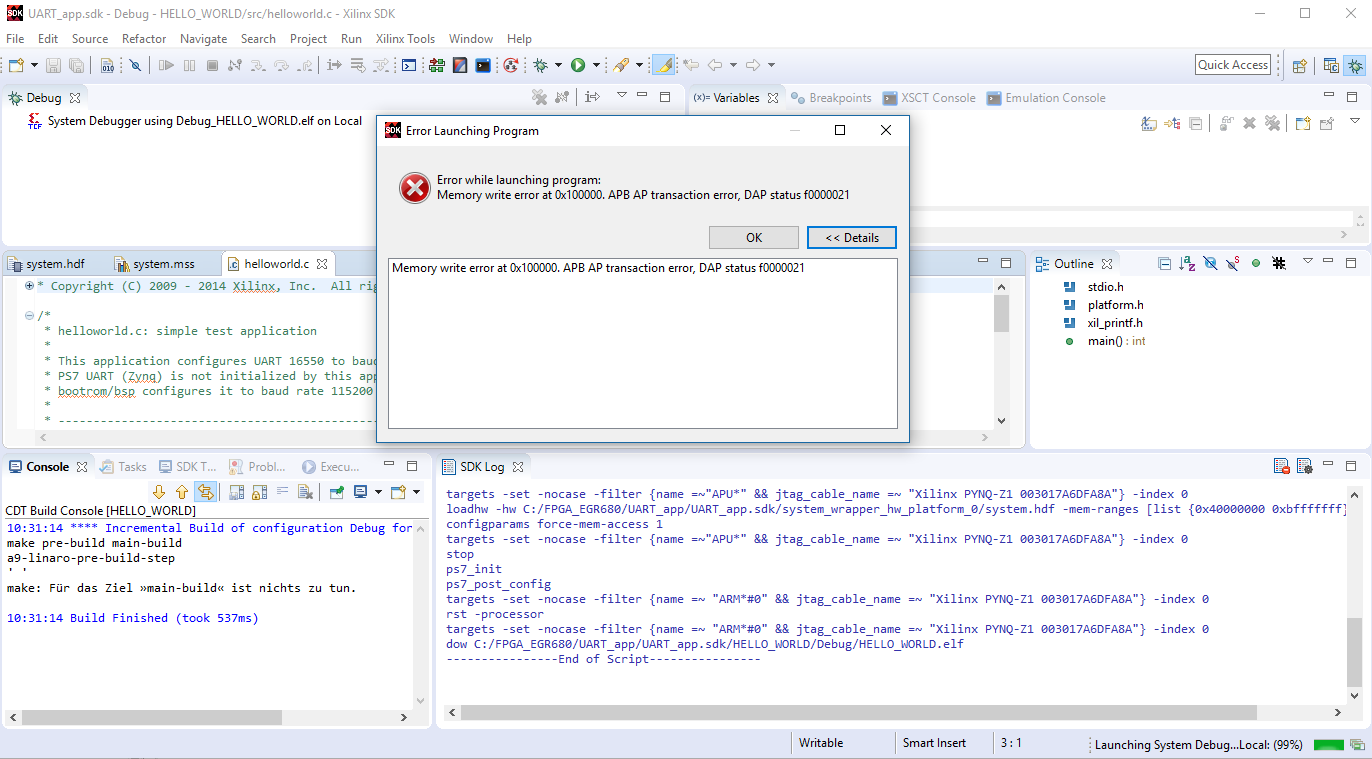
\includegraphics[width=1.0\textwidth]{01_images/Vivado_lab4_part1_SecondErrorSDK.PNG}
	\caption{Error SDK Part I.}
	\label{fig: Vivado_lab4_part1_SecondErrorSDK}
\end{figure}
%Verilog is used to describe a decoder that shall control a seven-segment display with two switches and one button. The given task is as followed:
%\\ \\
%The design should be implemented on t he PYNQ board using two Pmod 7-segment displays.
%VENDMACH is a vending machine that accepts nickels, and dimes, and dispenses gum, apple, or yogurt. A
%gum pack costs 10\cent, an apple is 15\cent, and yogurt is 20\cent. The machine is only allowed to accept up to 20\cent. Any
%coins inserted that pushes the value beyond 20\cent should be ignored.
%
%\begin{description}
%	\item[ - NICKEL]  \t a signal that becomes 1 when a nickel is deposited in the coin slot.
%	\item[ - DIME] a signal that becomes 1 when a dime is deposited in the coin slot.
%	\item[ - GUM] a signal that becomes 1 when the gum selection button is pressed.
%	\item[ - APPLE] a signal that becomes 1 when the apple select ion button is pressed.
%	\item[ - YOGURT] a signal that becomes 1 when the yogurt select ion button is pressed.
%\end{description}
%In addition ion to these “user” inputs, the machine has two control inputs:
%\begin{description}
%	\item[ - CLOCK] a timing signal that sequences the state transit ions of the machine.
%	\item[ - RST] an initialization signal that resets the machine to a suitable starting
%	state.
%\end{description}
%The machine has three outputs:
%\begin{description}
%	\item[ - MONEY ENTERED] The amount of money inserted into the machine should be displayed on one of the 7-segment Pmod displays. This should update every time a coin is inserted (i.e. 5\cent should read 05). Upon startup or reset, the display should read VEND.
%	\item[ - DISPENSED ITEM] The item that was just purchased should be displayed on the 7-segment: g for gum, A for apple, and y for yogurt, as indicated in figure below.
%	\item[ - CHANGE] The amount of money returned in change. The machine returns change using only	cents; the number of cents returned should be displayed as a binary number using the on-board LEDs.
%\end{description}
%
%
%\begin{figure}[H]
%	\centering
%	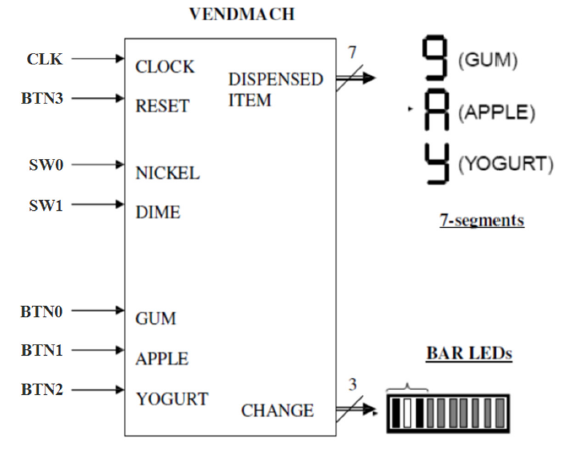
\includegraphics[width=0.7\textwidth]{01_images/Vivado_lab3_DesignSpec3_ModuleOverview.PNG}
%	\caption{VENDMACH top level module.}
%	\label{fig: Vivado_lab3_DesignSpec3_ModuleOverview}
%\end{figure}
%
%\subsection{Vending machine design description}\label{subsec: Vending machine design description}
%The above specification leads to the following table truth tables which can be used as aid to implement the logic in HDL. Table \ref{tab: VENDMACH allowed coins.} shows the logic relation between switch an coin. Table \ref{tab: VENDMACH products and prices.} shows the relation ship between button and product. 
%\subsubsection{Display}\label{subsubsec: Display}
%The knowledge that different values at different displays have to be shown lead to the idea of using an ASCII to seven-segment converter (ascii2seg) as separate module so in the state machine the actual out put can be represented as ASCII character. The ascii2seg output is routed in to the decoder that is based on a four to two MUX. The decoder is synchronized with a slower clk signal otherwise the display would not be visible. The state machine module has four character outputs theretofore the ascii2seg converter is build as module and used four times between state machine module and decoder.
%\subsubsection{De-bounce}\label{subsubsec: De-bounce}
%Input signals on the PYNQ-Z1 board are realized with switches and buttons that according to testing are not hardware de-bounced. This means that a button or switch has a ringing while the element switches from off to on state or from on state to off state. This can be easily encountered in software with a de-bouncer. The de-bouncer is realized with an two bit shift register and a state comparison between synchronized input and synchronized output that determines the output logic. To make it a denouncer the clock has to be slower then the ringing period of the switched element, so it uses a slow clock. The de-bouncer is implemented as module which allows the instantiation of the module for as many signals as have to be de-bounced. Notice, that because the de-bounce module uses a synchronous reset the reset button can not be de-bounced with it.
%
%\subsubsection{Edge detector}\label{subsubsec: Edge detector}
%After an input signal is de-bounced usually an edge detector is switched in serious that is build as the same as the de-bouncer but operates on the system clock to account for the faster switching past of the state machine (SM). Due to the fact that the Edge detector has the same clock as the SM it was implemented in the state machine file as in depended process in a synchronous always statement.
%
%\subsubsection{3 s Delay}\label{subsubsec: 3s Delay}
%A 3 s delay is used to keep the state after the vending process was successful that the display does not switch immediately to idle state. Therefor a simple counter was used to count up for $375*10^6$ ticks for a 125 MHz system clock used in the state machine. 
%
%\subsubsection{State Machine}\label{subsubsec: State Machine}
%The state machine is implemented in Moore Machine with an case statement synchronized on the the state value used for output logic. A second case statement is used to implement the logic flow depended on the given input states. The drawn  a bit simplified state machine is shown in figure \ref{fig: VNEDMACH state machine} therefore it can be easily used in the file as header which helps a lot by development on small screens. 
%\begin{table}[H]
%	\begin{center}
%		\begin{tabular}{|| c | c | c | c | c ||} 
%			\hline
%			  Description & Switches & Displayed Pmod A  \\ [0.5ex] 
%			\hline\hline
%			Nickel is 5 \cent 	& SW0 	& 	05  	\\ \hline
%			Dime is 10 \cent 	& SW1	&	10  	\\ \hline
%			
%		\end{tabular}
%	\end{center}
%	\caption{VENDMACH allowed coins.}\label{tab: VENDMACH allowed coins.}
%\end{table}
%
%\begin{table}[H]
%	\begin{center}
%		\begin{tabular}{|| c | c | c | c | c ||} 
%			\hline
%			Product & Price  & Displayed Pmod B \\ [0.5ex] 
%			\hline\hline
%			Gum  	& 10 \cent	& g		\\ \hline
%			Apple 	& 15 \cent	& A  	\\ \hline
%			Yogurt 	& 20 \cent	& y  	\\ \hline		
%		\end{tabular}
%	\end{center}
%	\caption{VENDMACH products and prices.} \label{tab: VENDMACH products and prices.}
%\end{table}
%\newpage
%\subsection{Vending machine State Machine}\label{subsec: Vending machine State Machin}
%\begin{figure}[H]
%	\begin{verbatim}       
%/*********************************************************************************
%** FSM State machine                                                            **
%**********************************************************************************
%                   000                                  
%+---------------------+               +---------------------+
%| Idle                |               |                     |
%| Display "VENT"      |<--------------| Reset               |<------+
%|                     |               | BTN3                |       |
%+---------------------+               +---------------------+-      |
%    |                                                               |
%    |                                                               |
%    |              002                                              |       001
%+---------------------+ Add to coin_val                  +---------------------+
%|                     |---------------+                  | Delay               |
%| Coin entered show   |               |                  | 3s                  |
%| coin_val on Pmod A  |<--------------+                  |                     |
%+---------------------+                                  +---------------------+
%    |                                                              / \ 
%    |                                                             / | \
%    |              003                                              |       006
%+---------------------+                                  +---------------------+
%| IF value > Gum      |                                  | Vend                |
%| & coin_val > 10     |--------------------------------->|                     |
%| Display 'g' by BTN0 |                                  | Disp returned cents |
%+---------------------+                                  +---------------------+
%   |                                                               / \ 
%   |                                                              / | \
%   |              004                                               |
%+---------------------+                                             |
%| IF value > Apple    |                                             |
%| & coin_val > 15     |------------------->------------------->-----+
%| Display 'A' by BTN1 |                                             |
%+---------------------+                                             |
%    |                                                               |
%    |                                                               |
%    |              005                                              |
%+---------------------+                                             |
%| IF value > Yogurt   |                                             |
%| & coin_val > 20     |------------------->------------------->-----+
%| Display 'y' by BTN2 |                                           
%+---------------------+            
%
%	\end{verbatim}
%	\caption{VNEDMACH state machine.}\label{fig: VNEDMACH state machine}
%\end{figure}
%
%\subsection{Recommended improvements for future work}\label{subsec: Recommended improvements for future work}
%\begin{enumerate}
%	\item It is highly recommended for the development process that simulation and original hardware is used simultaneously if possible. A lot of time was lost due to a simple bug that most likely would have been found easily if in early design states would have used the hardware as well instead of simulation. Furthermore, the module initialization should be done with labels so that the order of the module input signals does not matter.
%	\item The Edge detector should be implemented as independent module.
%	\item Decide if a signal shall be set with blocking or non blocking statement, but do not mix those among another.
%\end{enumerate}
%
%
%
%
%
